\documentclass[11pt,]{article}
\usepackage[left=1in,top=1in,right=1in,bottom=1in]{geometry}
\newcommand*{\authorfont}{\fontfamily{phv}\selectfont}
\usepackage[]{mathpazo}


  \usepackage[T1]{fontenc}
  \usepackage[utf8]{inputenc}



\usepackage{abstract}
\renewcommand{\abstractname}{}    % clear the title
\renewcommand{\absnamepos}{empty} % originally center

\renewenvironment{abstract}
 {{%
    \setlength{\leftmargin}{0mm}
    \setlength{\rightmargin}{\leftmargin}%
  }%
  \relax}
 {\endlist}

\makeatletter
\def\@maketitle{%
  \newpage
%  \null
%  \vskip 2em%
%  \begin{center}%
  \let \footnote \thanks
    {\fontsize{18}{20}\selectfont\raggedright  \setlength{\parindent}{0pt} \@title \par}%
}
%\fi
\makeatother




\setcounter{secnumdepth}{0}

\usepackage{color}
\usepackage{fancyvrb}
\newcommand{\VerbBar}{|}
\newcommand{\VERB}{\Verb[commandchars=\\\{\}]}
\DefineVerbatimEnvironment{Highlighting}{Verbatim}{commandchars=\\\{\}}
% Add ',fontsize=\small' for more characters per line
\usepackage{framed}
\definecolor{shadecolor}{RGB}{248,248,248}
\newenvironment{Shaded}{\begin{snugshade}}{\end{snugshade}}
\newcommand{\KeywordTok}[1]{\textcolor[rgb]{0.13,0.29,0.53}{\textbf{{#1}}}}
\newcommand{\DataTypeTok}[1]{\textcolor[rgb]{0.13,0.29,0.53}{{#1}}}
\newcommand{\DecValTok}[1]{\textcolor[rgb]{0.00,0.00,0.81}{{#1}}}
\newcommand{\BaseNTok}[1]{\textcolor[rgb]{0.00,0.00,0.81}{{#1}}}
\newcommand{\FloatTok}[1]{\textcolor[rgb]{0.00,0.00,0.81}{{#1}}}
\newcommand{\ConstantTok}[1]{\textcolor[rgb]{0.00,0.00,0.00}{{#1}}}
\newcommand{\CharTok}[1]{\textcolor[rgb]{0.31,0.60,0.02}{{#1}}}
\newcommand{\SpecialCharTok}[1]{\textcolor[rgb]{0.00,0.00,0.00}{{#1}}}
\newcommand{\StringTok}[1]{\textcolor[rgb]{0.31,0.60,0.02}{{#1}}}
\newcommand{\VerbatimStringTok}[1]{\textcolor[rgb]{0.31,0.60,0.02}{{#1}}}
\newcommand{\SpecialStringTok}[1]{\textcolor[rgb]{0.31,0.60,0.02}{{#1}}}
\newcommand{\ImportTok}[1]{{#1}}
\newcommand{\CommentTok}[1]{\textcolor[rgb]{0.56,0.35,0.01}{\textit{{#1}}}}
\newcommand{\DocumentationTok}[1]{\textcolor[rgb]{0.56,0.35,0.01}{\textbf{\textit{{#1}}}}}
\newcommand{\AnnotationTok}[1]{\textcolor[rgb]{0.56,0.35,0.01}{\textbf{\textit{{#1}}}}}
\newcommand{\CommentVarTok}[1]{\textcolor[rgb]{0.56,0.35,0.01}{\textbf{\textit{{#1}}}}}
\newcommand{\OtherTok}[1]{\textcolor[rgb]{0.56,0.35,0.01}{{#1}}}
\newcommand{\FunctionTok}[1]{\textcolor[rgb]{0.00,0.00,0.00}{{#1}}}
\newcommand{\VariableTok}[1]{\textcolor[rgb]{0.00,0.00,0.00}{{#1}}}
\newcommand{\ControlFlowTok}[1]{\textcolor[rgb]{0.13,0.29,0.53}{\textbf{{#1}}}}
\newcommand{\OperatorTok}[1]{\textcolor[rgb]{0.81,0.36,0.00}{\textbf{{#1}}}}
\newcommand{\BuiltInTok}[1]{{#1}}
\newcommand{\ExtensionTok}[1]{{#1}}
\newcommand{\PreprocessorTok}[1]{\textcolor[rgb]{0.56,0.35,0.01}{\textit{{#1}}}}
\newcommand{\AttributeTok}[1]{\textcolor[rgb]{0.77,0.63,0.00}{{#1}}}
\newcommand{\RegionMarkerTok}[1]{{#1}}
\newcommand{\InformationTok}[1]{\textcolor[rgb]{0.56,0.35,0.01}{\textbf{\textit{{#1}}}}}
\newcommand{\WarningTok}[1]{\textcolor[rgb]{0.56,0.35,0.01}{\textbf{\textit{{#1}}}}}
\newcommand{\AlertTok}[1]{\textcolor[rgb]{0.94,0.16,0.16}{{#1}}}
\newcommand{\ErrorTok}[1]{\textcolor[rgb]{0.64,0.00,0.00}{\textbf{{#1}}}}
\newcommand{\NormalTok}[1]{{#1}}
\usepackage{longtable,booktabs}

\usepackage{graphicx}
% We will generate all images so they have a width \maxwidth. This means
% that they will get their normal width if they fit onto the page, but
% are scaled down if they would overflow the margins.
\makeatletter
\def\maxwidth{\ifdim\Gin@nat@width>\linewidth\linewidth
\else\Gin@nat@width\fi}
\makeatother
\let\Oldincludegraphics\includegraphics
\renewcommand{\includegraphics}[1]{\Oldincludegraphics[width=\maxwidth]{#1}}

\title{Estatistica Descritiva - lista 3 \thanks{Replication files are available on the author's Github account
(\url{http://github.com/svmiller}). \textbf{Current version}: maio 24,
2017; \textbf{Corresponding author}:
\href{mailto:svmille@clemson.edu}{\nolinkurl{svmille@clemson.edu}}.}  }



\author{\Large Bruna Umino, Beatriz Vianna\vspace{0.05in} \newline\normalsize\emph{IME - USP}  }


\date{}

\usepackage{titlesec}

\titleformat*{\section}{\normalsize\bfseries}
\titleformat*{\subsection}{\normalsize\itshape}
\titleformat*{\subsubsection}{\normalsize\itshape}
\titleformat*{\paragraph}{\normalsize\itshape}
\titleformat*{\subparagraph}{\normalsize\itshape}


\usepackage{natbib}
\bibliographystyle{apsr}



\newtheorem{hypothesis}{Hypothesis}
\usepackage{setspace}

\makeatletter
\@ifpackageloaded{hyperref}{}{%
\ifxetex
  \usepackage[setpagesize=false, % page size defined by xetex
              unicode=false, % unicode breaks when used with xetex
              xetex]{hyperref}
\else
  \usepackage[unicode=true]{hyperref}
\fi
}
\@ifpackageloaded{color}{
    \PassOptionsToPackage{usenames,dvipsnames}{color}
}{%
    \usepackage[usenames,dvipsnames]{color}
}
\makeatother
\hypersetup{breaklinks=true,
            bookmarks=true,
            pdfauthor={Bruna Umino, Beatriz Vianna (IME - USP)},
             pdfkeywords = {pandoc, r markdown, knitr},  
            pdftitle={Estatistica Descritiva - lista 3},
            colorlinks=true,
            citecolor=blue,
            urlcolor=blue,
            linkcolor=magenta,
            pdfborder={0 0 0}}
\urlstyle{same}  % don't use monospace font for urls



\begin{document}
	
% \pagenumbering{arabic}% resets `page` counter to 1 
%
% \maketitle

{% \usefont{T1}{pnc}{m}{n}
\setlength{\parindent}{0pt}
\thispagestyle{plain}
{\fontsize{18}{20}\selectfont\raggedright 
\maketitle  % title \par  

}

{
   \vskip 13.5pt\relax \normalsize\fontsize{11}{12} 
\textbf{\authorfont Bruna Umino, Beatriz Vianna} \hskip 15pt \emph{\small IME - USP}   

}

}







\begin{abstract}

    \hbox{\vrule height .2pt width 39.14pc}

    \vskip 8.5pt % \small 

\noindent professora Marcia D'Elia Branco


\vskip 8.5pt \noindent \emph{Keywords}: pandoc, r markdown, knitr \par

    \hbox{\vrule height .2pt width 39.14pc}



\end{abstract}


\vskip 6.5pt

\noindent  \section{Questão 1}\label{questao-1}

\begin{Shaded}
\begin{Highlighting}[]
\NormalTok{ano<-}\KeywordTok{c}\NormalTok{(}\DecValTok{1942}\NormalTok{,}\DecValTok{1943}\NormalTok{,}\DecValTok{1944}\NormalTok{,}\DecValTok{1945}\NormalTok{,}\DecValTok{1946}\NormalTok{,}\DecValTok{1947}\NormalTok{,}\DecValTok{1948}\NormalTok{,}\DecValTok{1949}\NormalTok{,}\DecValTok{1950}\NormalTok{,}\DecValTok{1951}\NormalTok{,}
       \DecValTok{1952}\NormalTok{,}\DecValTok{1953}\NormalTok{,}\DecValTok{1954}\NormalTok{,}\DecValTok{1955}\NormalTok{,}\DecValTok{1956}\NormalTok{,}\DecValTok{1957}\NormalTok{,}\DecValTok{1958}\NormalTok{,}\DecValTok{1959}\NormalTok{,}\DecValTok{1960}\NormalTok{,}\DecValTok{1961}\NormalTok{)}

\NormalTok{colheita<-}\KeywordTok{c}\NormalTok{(}\DecValTok{6409}\NormalTok{, }\DecValTok{19835}\NormalTok{, }\DecValTok{10939}\NormalTok{, }\DecValTok{7826}\NormalTok{, }\DecValTok{7165}\NormalTok{, }\DecValTok{7807}\NormalTok{, }\DecValTok{6028}\NormalTok{, }\DecValTok{6037}\NormalTok{, }\DecValTok{6458}\NormalTok{, }\DecValTok{6981}\NormalTok{,}
            \DecValTok{4233}\NormalTok{, }\DecValTok{8790}\NormalTok{, }\DecValTok{8959}\NormalTok{, }\DecValTok{8289}\NormalTok{, }\DecValTok{7910}\NormalTok{, }\DecValTok{6775}\NormalTok{, }\DecValTok{6088}\NormalTok{, }\DecValTok{6381}\NormalTok{, }\DecValTok{8600}\NormalTok{, }\DecValTok{4805}\NormalTok{)}

\NormalTok{preco<-}\KeywordTok{c}\NormalTok{(}\FloatTok{2.26}\NormalTok{, }\FloatTok{1.64}\NormalTok{, }\FloatTok{1.52}\NormalTok{, }\FloatTok{2.29}\NormalTok{, }\FloatTok{3.54}\NormalTok{, }\FloatTok{2.09}\NormalTok{, }\FloatTok{2.46}\NormalTok{, }\FloatTok{2.50}\NormalTok{, }\FloatTok{2.62}\NormalTok{, }\FloatTok{2.57}\NormalTok{,}
         \FloatTok{3.38}\NormalTok{, }\FloatTok{2.02}\NormalTok{, }\FloatTok{1.68}\NormalTok{, }\FloatTok{1.78}\NormalTok{, }\FloatTok{1.99}\NormalTok{, }\FloatTok{3.02}\NormalTok{, }\FloatTok{3.23}\NormalTok{, }\FloatTok{2.98}\NormalTok{, }\FloatTok{2.74}\NormalTok{, }\FloatTok{3.38}\NormalTok{)}
\NormalTok{tabela <-}\StringTok{ }\KeywordTok{data.frame}\NormalTok{(ano, colheita, preco)}
\end{Highlighting}
\end{Shaded}

\section{1a)}\label{a}

\begin{Shaded}
\begin{Highlighting}[]
\CommentTok{#Grafico de dispersao}
\KeywordTok{plot}\NormalTok{( preco ~}\StringTok{ }\NormalTok{colheita, }
      \DataTypeTok{xlab =} \StringTok{"Colheita (em milhares de hectolitros)"}\NormalTok{,}
      \DataTypeTok{ylab =} \StringTok{"Preço (escudos/litro)"}\NormalTok{,}
      \DataTypeTok{main =} \StringTok{"Gráfico de dispersão"}\NormalTok{)}
\end{Highlighting}
\end{Shaded}

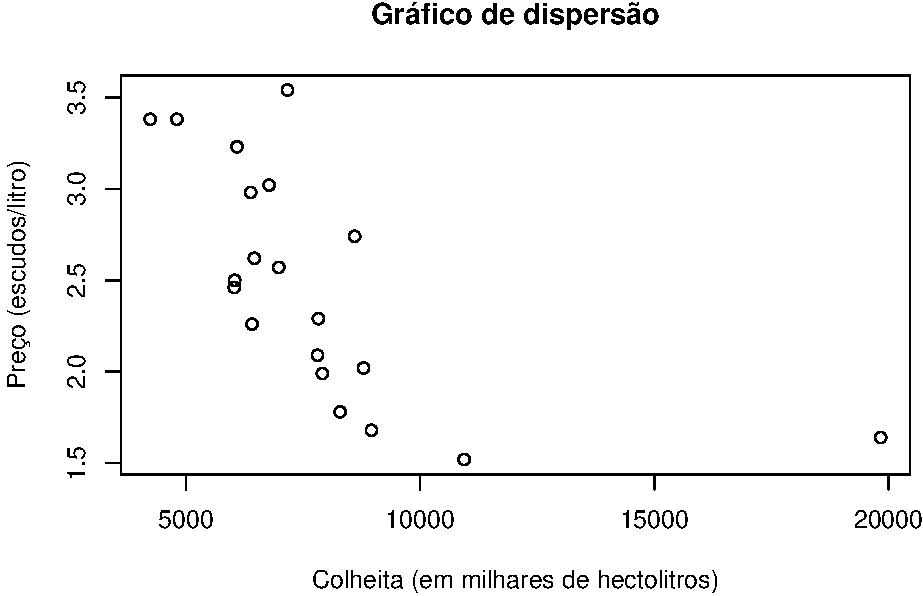
\includegraphics{versaofinal_lista3_files/figure-latex/unnamed-chunk-2-1.pdf}

\begin{Shaded}
\begin{Highlighting}[]
\CommentTok{#Correlacao linear }
\KeywordTok{cor}\NormalTok{(preco, colheita)}
\end{Highlighting}
\end{Shaded}

\begin{verbatim}
## [1] -0.6239457
\end{verbatim}

Como podemos observar, o gráfico apresenta uma correlação linear
significativa e negativa (ou seja, quanto menor a colheita, mais alto
fica o preço), que está sendo influenciada pelo dado do ano de 1943.
Devido a este valor, a correlação está mais elevada.

\section{1b)}\label{b}

\begin{Shaded}
\begin{Highlighting}[]
\KeywordTok{plot}\NormalTok{( preco ~}\StringTok{ }\NormalTok{colheita, }
      \DataTypeTok{xlab =} \StringTok{"Colheita (em milhares de hectolitros)"}\NormalTok{,}
      \DataTypeTok{ylab =} \StringTok{"Preço (escudos/litro)"}\NormalTok{,}
      \DataTypeTok{main =} \StringTok{"Gráfico de dispersão com reta de regressão"}\NormalTok{)}
\KeywordTok{abline}\NormalTok{(}\KeywordTok{lm} \NormalTok{(preco ~}\StringTok{ }\NormalTok{colheita))}
\end{Highlighting}
\end{Shaded}

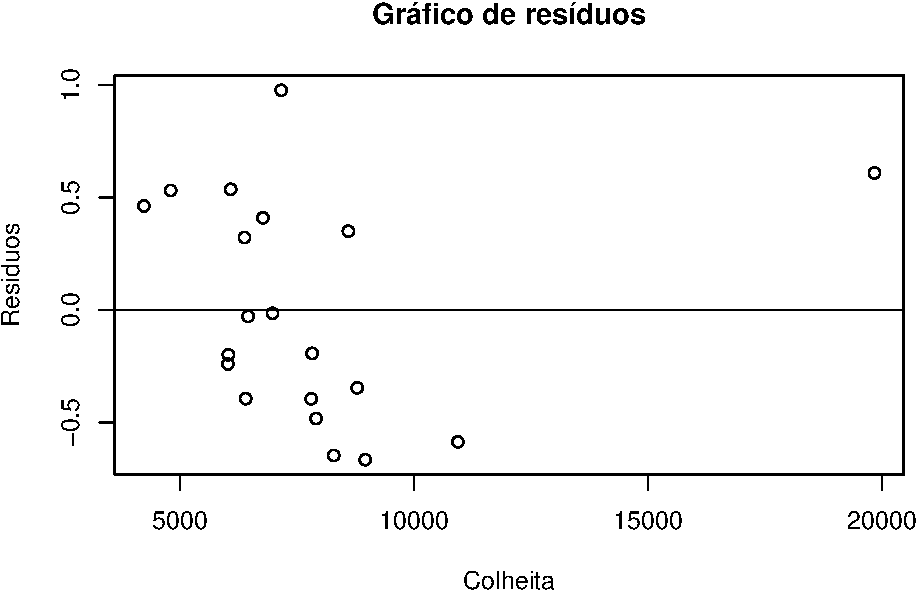
\includegraphics{versaofinal_lista3_files/figure-latex/unnamed-chunk-4-1.pdf}

\begin{Shaded}
\begin{Highlighting}[]
\KeywordTok{lm} \NormalTok{(preco ~}\StringTok{ }\NormalTok{colheita)}
\end{Highlighting}
\end{Shaded}

\begin{verbatim}
## 
## Call:
## lm(formula = preco ~ colheita)
## 
## Coefficients:
## (Intercept)     colheita  
##   3.4297758   -0.0001209
\end{verbatim}

Dado que o resultado do coeficiente angular foi igual a -0.0001209,
podemos observar que consiste em um valor negativo, ou seja, o preço e a
colheita são inversamente proporcionais.

\section{1c)}\label{c}

\begin{Shaded}
\begin{Highlighting}[]
\KeywordTok{lm}\NormalTok{(preco~colheita)}
\end{Highlighting}
\end{Shaded}

\begin{verbatim}
## 
## Call:
## lm(formula = preco ~ colheita)
## 
## Coefficients:
## (Intercept)     colheita  
##   3.4297758   -0.0001209
\end{verbatim}

\begin{Shaded}
\begin{Highlighting}[]
\NormalTok{residuos <-}\StringTok{ }\KeywordTok{resid}\NormalTok{(}\KeywordTok{lm}\NormalTok{(preco~colheita))}
\KeywordTok{plot}\NormalTok{(colheita, residuos,}
     \DataTypeTok{ylab=}\StringTok{"Residuos"}\NormalTok{,}
     \DataTypeTok{xlab=}\StringTok{"Colheita"}\NormalTok{,}
     \DataTypeTok{main=}\StringTok{"Gráfico de resíduos"}\NormalTok{) }
\KeywordTok{abline}\NormalTok{(}\DecValTok{0}\NormalTok{,}\DecValTok{0}\NormalTok{)}
\end{Highlighting}
\end{Shaded}

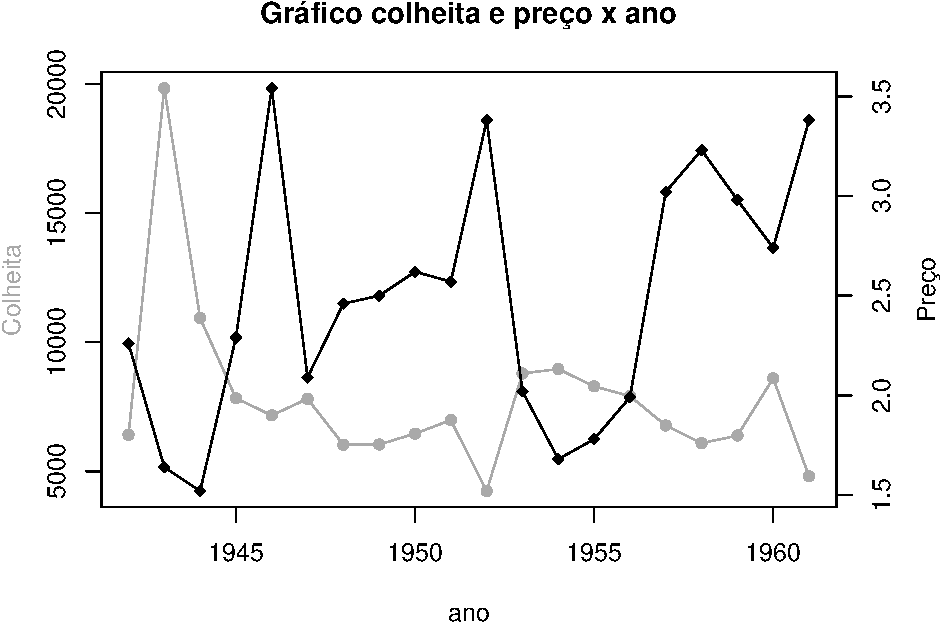
\includegraphics{versaofinal_lista3_files/figure-latex/unnamed-chunk-5-1.pdf}

Observando o gráfico, podemos ver que aumentando o valor da colheita,
não aumenta a variabilidade dos dados, então o gráfico é homocedástico.

\section{1d)}\label{d}

\begin{Shaded}
\begin{Highlighting}[]
\KeywordTok{par}\NormalTok{(}\DataTypeTok{mar=}\KeywordTok{c}\NormalTok{(}\DecValTok{4}\NormalTok{,}\DecValTok{4}\NormalTok{,}\DecValTok{4}\NormalTok{,}\DecValTok{4}\NormalTok{))}
\CommentTok{#grafico de dispersão ano x colheita}
\KeywordTok{plot} \NormalTok{(colheita~ano, }\DataTypeTok{type=}\StringTok{"o"}\NormalTok{, }\DataTypeTok{col=}\StringTok{"darkgray"}\NormalTok{, }\DataTypeTok{ylab =} \StringTok{""}\NormalTok{, }\DataTypeTok{pch=}\DecValTok{16}\NormalTok{,}
      \DataTypeTok{main =} \StringTok{"Gráfico colheita x ano x preço"}\NormalTok{)}
\KeywordTok{mtext}\NormalTok{(}\StringTok{"Colheita"}\NormalTok{, }\DataTypeTok{side =} \DecValTok{2}\NormalTok{, }\DataTypeTok{line =} \FloatTok{2.5}\NormalTok{, }\DataTypeTok{col=}\StringTok{"darkgray"}\NormalTok{)}
\KeywordTok{par}\NormalTok{(}\DataTypeTok{new=}\OtherTok{TRUE}\NormalTok{)}
\CommentTok{#grafico de dispersão ano x preço}
\KeywordTok{plot}\NormalTok{(preco~ano, }\DataTypeTok{axes=}\OtherTok{FALSE}\NormalTok{, }\DataTypeTok{type=}\StringTok{'o'}\NormalTok{, }\DataTypeTok{col=}\StringTok{'black'}\NormalTok{, }\DataTypeTok{ann=}\OtherTok{FALSE}\NormalTok{, }\DataTypeTok{pch=}\DecValTok{18}\NormalTok{)}
\KeywordTok{mtext}\NormalTok{(}\StringTok{"Preço"}\NormalTok{, }\DataTypeTok{side =} \DecValTok{4}\NormalTok{, }\DataTypeTok{line =} \FloatTok{2.5}\NormalTok{, }\DataTypeTok{col=}\StringTok{"black"}\NormalTok{)}
\KeywordTok{axis}\NormalTok{(}\DecValTok{4}\NormalTok{)}
\end{Highlighting}
\end{Shaded}

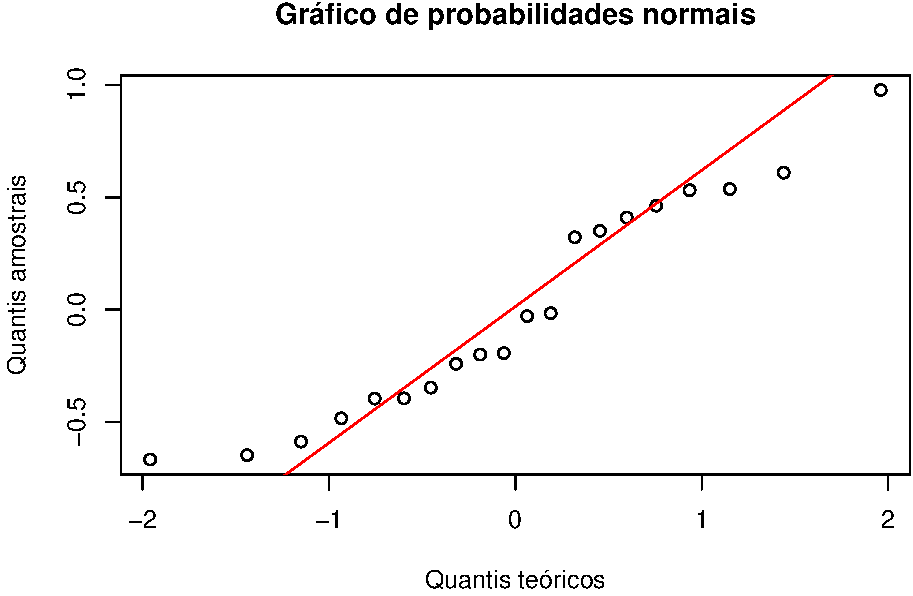
\includegraphics{versaofinal_lista3_files/figure-latex/unnamed-chunk-6-1.pdf}
Através dos gráficos podemos observar que ocoreu uma considerável
colheita no ano de 1943, que resultou no pior preço e no ano de 1952
ocorreu a menor colheita deste intervalo de tempo. O resto dos valores
coletados está na faixa de 5000 a 10900 milhares de hectolitros. Em
relação ao preço, há picos nos anos de 1946, 1961, 1952 e 1958, que são
os anos nos quais ocorreram as piores colheitas, e nos anos de 1944,
1943 e 1954, quando foram relatados os menores preços.

\section{1e)}\label{e}

\begin{Shaded}
\begin{Highlighting}[]
\KeywordTok{qqnorm}\NormalTok{(residuos, }
       \DataTypeTok{main =} \StringTok{"Gráfico de probabilidades normais"}\NormalTok{, }
       \DataTypeTok{xlab =} \StringTok{"Quantis teóricos"}\NormalTok{, }
       \DataTypeTok{ylab =} \StringTok{"Quantis amostrais"}\NormalTok{)}
\KeywordTok{qqline}\NormalTok{(residuos, }\DataTypeTok{col=}\StringTok{"red"}\NormalTok{)}
\end{Highlighting}
\end{Shaded}

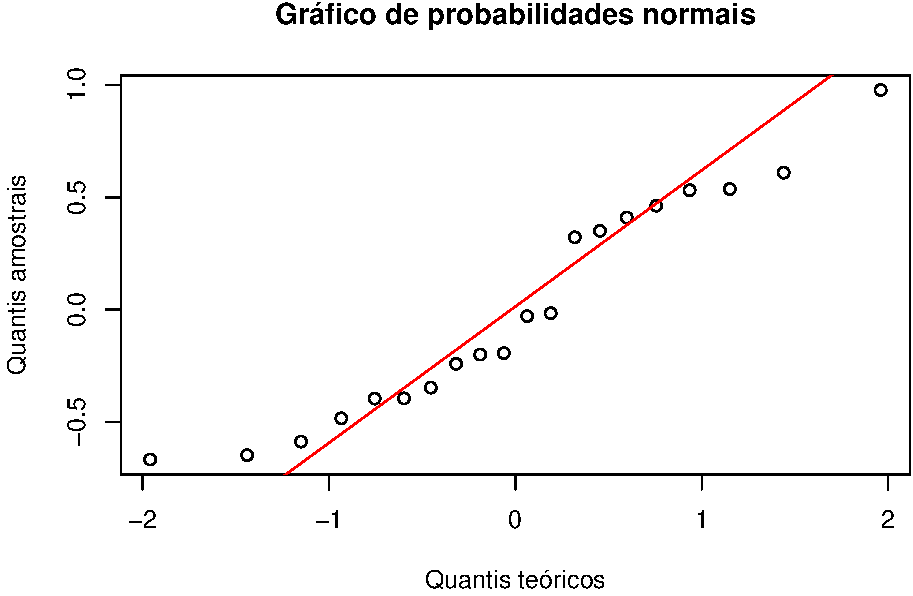
\includegraphics{versaofinal_lista3_files/figure-latex/unnamed-chunk-7-1.pdf}
Os quantis dos resíduos não se aproximam muito para uma normal, mas
podemos observar que os valores do meio estão mais próximos da linha
\(Y=X\) e as caudas se afastam consideravelmente. --- \#Questao 2

\section{2a)}\label{a-1}

\begin{Shaded}
\begin{Highlighting}[]
\KeywordTok{library} \NormalTok{(magrittr)}
\NormalTok{dados <-}\StringTok{ }\KeywordTok{read.csv2}\NormalTok{(}\StringTok{"/home/be/viabianna/Downloads/dadosmalariaCEA15P14.csv"}\NormalTok{)}
\CommentTok{#Retirar os dados que contém N/A}
\NormalTok{dados %>%}\StringTok{ }\KeywordTok{subset}\NormalTok{(!}\KeywordTok{is.na}\NormalTok{(pc)) %>%}\StringTok{ }\KeywordTok{subset}\NormalTok{(!}\KeywordTok{is.na}\NormalTok{(peso)) %>%}\StringTok{ }\KeywordTok{subset}\NormalTok{(!}\KeywordTok{is.na}\NormalTok{(est))}
\end{Highlighting}
\end{Shaded}

\begin{Shaded}
\begin{Highlighting}[]
\CommentTok{#Gráfico de Dispersão Perímetro Cefálico x Peso}
\KeywordTok{plot}\NormalTok{(dados$pc~dados$peso, }\DataTypeTok{xlab=}\StringTok{"Perímetro Cefálico"}\NormalTok{, }\DataTypeTok{ylab=}\StringTok{"Peso"}\NormalTok{,}
     \DataTypeTok{main=} \StringTok{"Gráfico de Dispersão Perímetro Cefálico x Peso"}\NormalTok{)}
\end{Highlighting}
\end{Shaded}

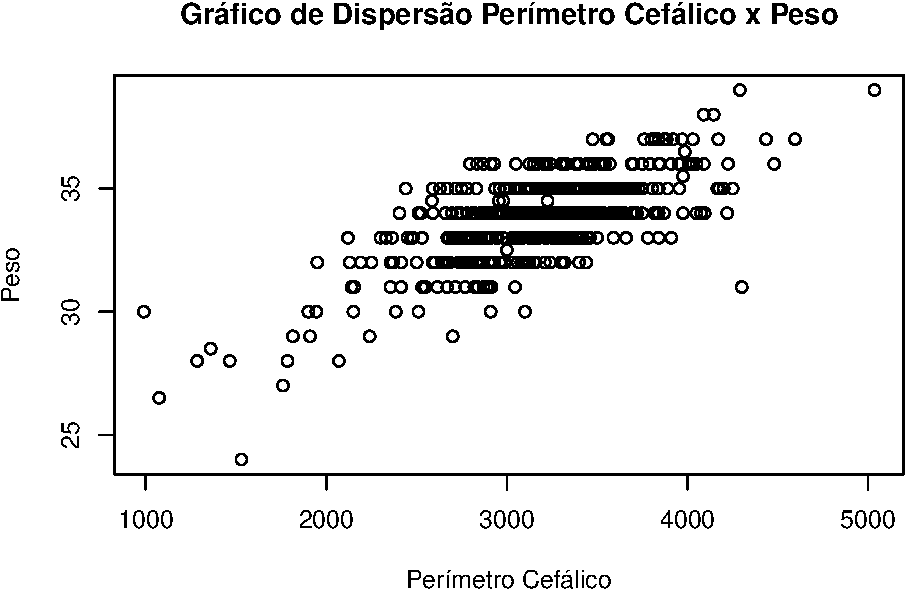
\includegraphics{versaofinal_lista3_files/figure-latex/unnamed-chunk-9-1.pdf}

\begin{Shaded}
\begin{Highlighting}[]
\CommentTok{#Correlação Perímetro Cefálico x Peso}
\KeywordTok{cor}\NormalTok{(dados$pc,dados$peso)}
\end{Highlighting}
\end{Shaded}

\begin{verbatim}
## [1] NA
\end{verbatim}

\begin{Shaded}
\begin{Highlighting}[]
\CommentTok{#Gráfico de Dispersão Perímetro Cefálico x Estatura}
\KeywordTok{plot}\NormalTok{(dados$pc~dados$est, }\DataTypeTok{xlab=}\StringTok{"Perímetro Cefálico"}\NormalTok{, }\DataTypeTok{ylab=}\StringTok{"Estatura"}\NormalTok{,}
     \DataTypeTok{main=} \StringTok{"Gráfico de Dispersão Perímetro Cefálico x Estatura"}\NormalTok{)}
\end{Highlighting}
\end{Shaded}

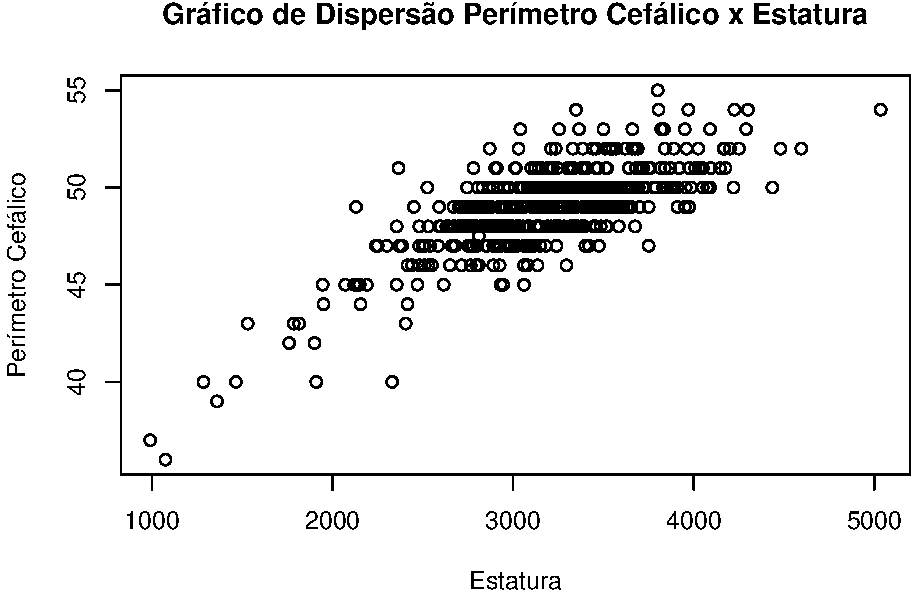
\includegraphics{versaofinal_lista3_files/figure-latex/unnamed-chunk-9-2.pdf}

\begin{Shaded}
\begin{Highlighting}[]
\CommentTok{#Correlação Perímetro Cefálico x Estatura}
\KeywordTok{cor}\NormalTok{(dados$pc,dados$est)}
\end{Highlighting}
\end{Shaded}

\begin{verbatim}
## [1] NA
\end{verbatim}

\section{2b)}\label{b-1}

\begin{Shaded}
\begin{Highlighting}[]
\NormalTok{equação <-}\StringTok{ }\NormalTok{(}\KeywordTok{lm}\NormalTok{(dados$pc~dados$peso))}
\NormalTok{equação}
\end{Highlighting}
\end{Shaded}

\begin{verbatim}
## 
## Call:
## lm(formula = dados$pc ~ dados$peso)
## 
## Coefficients:
## (Intercept)   dados$peso  
##    26.06791      0.00244
\end{verbatim}

A partir destes dados, sabemos que a reta de regressão para Perímetro
Cefálico x Peso (que é a variável que apresenta maior correlação) será

\(y = 0.002x + 26.061\)

portanto, o perímetro cefálico, em centímetros, esperado para um bebê de
3000g é:

\(y= 0.002*3000 + 26.061\)

\(y= 32.061\)

\begin{Shaded}
\begin{Highlighting}[]
\NormalTok{equação <-}\StringTok{ }\NormalTok{(}\KeywordTok{lm}\NormalTok{(dados$pc~dados$est))}
\NormalTok{equação}
\end{Highlighting}
\end{Shaded}

\begin{verbatim}
## 
## Call:
## lm(formula = dados$pc ~ dados$est)
## 
## Coefficients:
## (Intercept)    dados$est  
##     10.2103       0.4824
\end{verbatim}

Já a reta Perímetro Cefálico x Estatura (que apresenta menor correlação)
será

\(y=0.482x + 10.21\)

Assim sendo, o perímetro cefálico esperado, em centímetros, para um
recém nascido de 50cm será:

\(y= 0.482 * 50 + 10.21\)

\(y= 34.31\) \#2c)

\begin{Shaded}
\begin{Highlighting}[]
\CommentTok{#organização dos dados a serem usados,}
\CommentTok{#transformar grupo em variável binária}
\NormalTok{dados2 <-}\StringTok{ }\KeywordTok{data.frame}\NormalTok{(dados$peso, dados$grupo, dados$pc)}
\NormalTok{dadosgrupo <-}\StringTok{ }\KeywordTok{vector}\NormalTok{(}\DataTypeTok{length=}\KeywordTok{length}\NormalTok{(dados2$dados.grupo))}
\NormalTok{dadosgrupo[}\KeywordTok{which}\NormalTok{(dados2$dados.grupo!=}\DecValTok{0}\NormalTok{)] <-}\StringTok{ 'Infectada'}
\NormalTok{dadosgrupo[}\KeywordTok{which}\NormalTok{(dados2$dados.grupo==}\DecValTok{0}\NormalTok{)] <-}\StringTok{ "Não Infectada"}
\NormalTok{dados2$dados.grupo <-}\StringTok{ }\NormalTok{dadosgrupo}
\end{Highlighting}
\end{Shaded}

\begin{Shaded}
\begin{Highlighting}[]
\KeywordTok{library}\NormalTok{(ggplot2)}
\NormalTok{legenda <-}\StringTok{ }\KeywordTok{as.factor}\NormalTok{(dados2$dados.grupo)}
\KeywordTok{ggplot}\NormalTok{(}\DataTypeTok{data =} \NormalTok{dados2, }
      \KeywordTok{aes}\NormalTok{(}\DataTypeTok{x =} \NormalTok{dados2$dados.pc, }\DataTypeTok{y =}\NormalTok{dados2$dados.peso, }\DataTypeTok{colour =} \NormalTok{legenda)) +}
\StringTok{      }\KeywordTok{geom_point}\NormalTok{()+}
\StringTok{      }\KeywordTok{xlab}\NormalTok{(}\StringTok{"Perímetro Cefálico"}\NormalTok{)+}
\StringTok{      }\KeywordTok{ylab}\NormalTok{(}\StringTok{"Peso"}\NormalTok{)+}
\StringTok{      }\KeywordTok{labs}\NormalTok{(}\DataTypeTok{title=}\StringTok{"Gráfico de Dispersão Perímetro Cefálico x Peso"}\NormalTok{)}
\end{Highlighting}
\end{Shaded}

\begin{verbatim}
## Warning: Removed 70 rows containing missing values (geom_point).
\end{verbatim}

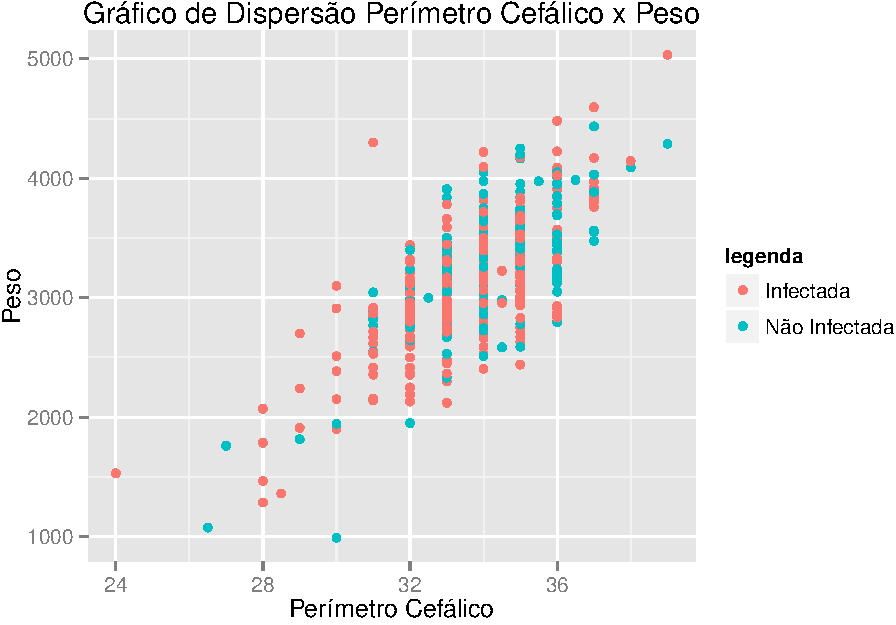
\includegraphics{versaofinal_lista3_files/figure-latex/unnamed-chunk-13-1.pdf}

\section{2d)}\label{d-1}

\begin{Shaded}
\begin{Highlighting}[]
\CommentTok{#organização dos dados a serem utilizados, transformar grupo em binário}
\CommentTok{#transformar idade em binária (maior que 35/ menor ou igual a 35)}
\NormalTok{dados3 <-}\StringTok{ }\KeywordTok{data.frame}\NormalTok{( dados$grupo, dados$pc, dados$idade)}
\NormalTok{dadosgrupo <-}\StringTok{ }\KeywordTok{vector}\NormalTok{(}\DataTypeTok{length=}\KeywordTok{length}\NormalTok{(dados3$dados.grupo))}
\NormalTok{dadosgrupo[}\KeywordTok{which}\NormalTok{(dados3$dados.grupo!=}\DecValTok{0}\NormalTok{)] <-}\StringTok{ }\DecValTok{1}
\NormalTok{dados3$dados.grupo <-}\StringTok{ }\NormalTok{dadosgrupo}
\NormalTok{dadosgrupo2 <-}\StringTok{ }\KeywordTok{vector}\NormalTok{(}\DataTypeTok{length=}\KeywordTok{length}\NormalTok{(dados3$dados.idade))}
\NormalTok{dadosgrupo2[}\KeywordTok{which}\NormalTok{(dados3$dados.idade<=}\DecValTok{35}\NormalTok{)] <-}\StringTok{ }\DecValTok{0}
\NormalTok{dadosgrupo2[}\KeywordTok{which}\NormalTok{(dados3$dados.idade>}\DecValTok{35}\NormalTok{)] <-}\StringTok{ }\DecValTok{1}
\NormalTok{dados3$idadecat<-}\StringTok{ }\NormalTok{dadosgrupo2}
\end{Highlighting}
\end{Shaded}

\begin{Shaded}
\begin{Highlighting}[]
\NormalTok{fit1 <-}\StringTok{ }\KeywordTok{lm}\NormalTok{(dados3$dados.pc~dados3$dados.grupo+dados3$idadecat)}
\KeywordTok{summary}\NormalTok{(fit1)}
\end{Highlighting}
\end{Shaded}

\begin{verbatim}
## 
## Call:
## lm(formula = dados3$dados.pc ~ dados3$dados.grupo + dados3$idadecat)
## 
## Residuals:
##    Min     1Q Median     3Q    Max 
## -9.616 -1.063  0.384  1.384  5.384 
## 
## Coefficients:
##                    Estimate Std. Error t value Pr(>|t|)    
## (Intercept)         34.0626     0.1240 274.756  < 2e-16 ***
## dados3$dados.grupo  -0.4467     0.1561  -2.861  0.00439 ** 
## dados3$idadecat      0.4748     0.3728   1.273  0.20342    
## ---
## Signif. codes:  0 '***' 0.001 '**' 0.01 '*' 0.05 '.' 0.1 ' ' 1
## 
## Residual standard error: 1.747 on 527 degrees of freedom
##   (70 observations deleted due to missingness)
## Multiple R-squared:  0.01885,    Adjusted R-squared:  0.01512 
## F-statistic: 5.062 on 2 and 527 DF,  p-value: 0.006647
\end{verbatim}

\begin{Shaded}
\begin{Highlighting}[]
\KeywordTok{par}\NormalTok{(}\DataTypeTok{mfrow=}\KeywordTok{c}\NormalTok{(}\DecValTok{2}\NormalTok{,}\DecValTok{2}\NormalTok{))}
\KeywordTok{plot}\NormalTok{(fit1, }\DataTypeTok{caption =} \KeywordTok{c}\NormalTok{(}\StringTok{"Resíduos x Ajustados"}\NormalTok{, }\StringTok{"QQ-Plot Normal"}\NormalTok{,}
                       \StringTok{"Locação e Escala"}\NormalTok{, }\StringTok{"resìduos e alavancagem"}\NormalTok{))}
\end{Highlighting}
\end{Shaded}

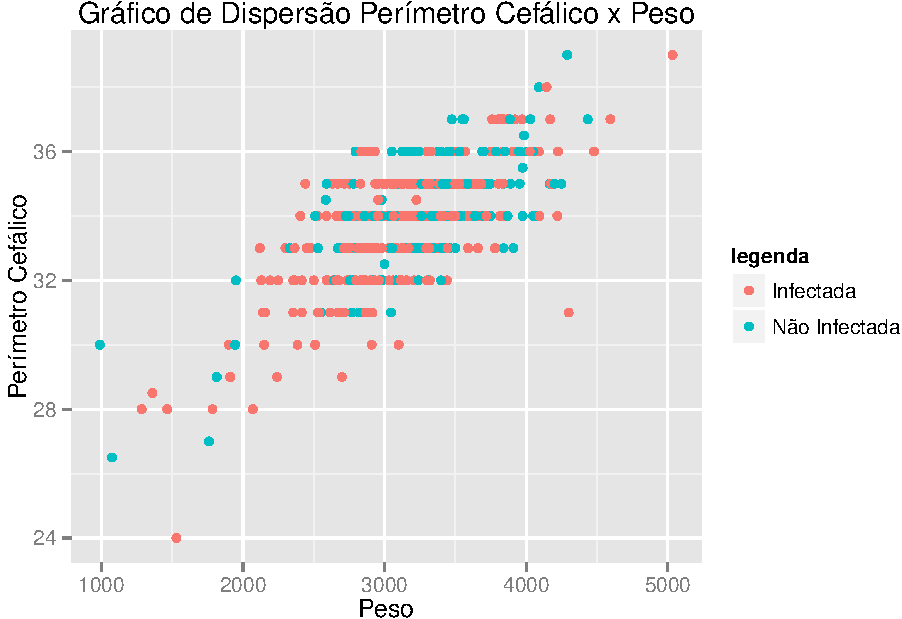
\includegraphics{versaofinal_lista3_files/figure-latex/unnamed-chunk-15-1.pdf}

O modelo está ajustando o perímetro cefálico em relação ao grupo da
gestante (0=não infectada e 1=infectada) e a idade da gestante (0= até
35 anos e 1=mais de 35 anos)

O desvio padrão dos resíduos é 1.748

Devido aos dados estarem agrupados de forma binária, os gráficos com
exceção do qqnorm saem alinhados verticalmente. Em relação ao gráfico de
residuos podemos observar que a medida que aumenta o eixo x (a idade e o
grupo), diminui a variabilidade dos dados, mostrando uma não
homocedastidade. No entanto, analisando o gráfico qqnorm, o modelo se
aproxima de uma normal, exceto nas caudas.

\begin{center}\rule{0.5\linewidth}{\linethickness}\end{center}

\section{Questão 3}\label{questao-3}

 Ao se fazer um diagnóstico binário, no qual Y assume apenas dois
valores (positivo e negativo), queremos uma regra de predição que
minimize os erros cometidos. Se tomarmos \(\pi =1\) por exemplo, nosso Y
sempre será positivo. Isso irá maximizar o diagnóstico de verdadeiros
positivos, mas também irá minimizar o diagnóstico dos quadros negativos,
ou seja, também teremos muitos falsos positivos (valores negativos que
foram diagnosticados erroneamente como positivos).

Para a escolha do valor de pi é utilizada a curva ROC (do inglês
Receiver Operating Characteristic - Característica de operação do
receptor). Este gráfico apresenta em seu eixo vertical
P(Y=1\textbar{}Y=1) - chamado sensibilidade - e em seu eixo horizontal
1-P(Y=0\textbar{}Y=0) - chamado especificidade. A curva apresenta a
associação entre as duas variáveis (sensibilidade e especificidade) para
cada valor de pi entre 0 e 1. O que procuramos é o ponto da curva que
apresenta um valor muito alto para a variável do eixo y e um muito baixo
para a variável do eixo x.

\begin{longtable}[]{@{}lll@{}}
\toprule
Resultado do teste sob investigação & positivos &
negativos\tabularnewline
\midrule
\endhead
positivo & verdadeiros positivos & falsos positivos\tabularnewline
negativo & falsos negativos & verdadeiros negativos\tabularnewline
total & total positivos & total negativos\tabularnewline
------ & ------ & ------\tabularnewline
desempenho & sensibilidade & especificidade\tabularnewline
\bottomrule
\end{longtable}

\newpage
\singlespacing 
\bibliography{/home/be/viabianna/Dropbox/master.bib}

\end{document}
